\section{Architecture and design}\label{sec:archdesign}

This section describes the architecture and design behind our solution using text and illustrative UML diagrams defined the methodology. The section will give the reader an overview of which parts of the application are modeled and mapped to hardware, and which are kept purely in software.

\subsection{Architecture of components}

The overall structure of the system can be seen in the block definition diagram in figure \ref{fig:bdd}, as the system should consist of mainly three parts: \emph{User Interface}, \emph{GenerationGenerator}, and \emph{Simulator}. Each part has a responsibility within a scope and could potentially be placed in either hardware or software. We will now briefly review the three:

\emph{User Interface} is what the user sees and interacts with via a console. The software part is responsible for getting the input from the user and send output back, e.g. the start generation of chromosomes, a continuous loop of fitnesses by evaluating future chromosomes and the final one for the function.
\emph{GenerationGenerator} is responsible for generating a new generation of chromosomes using the genetic algorithm by doing crossovers and mutation on the basis of some stochastic probability.
\emph{Simulator} is responsible for calculating the fitness of a chromosomes in a generation using the Rosenbrock function by evaluating it given $x_{i}$ and $y_{i}$. The result is a measure of how close we are to the minimum.

\begin{figure}[h!]
	\centering
	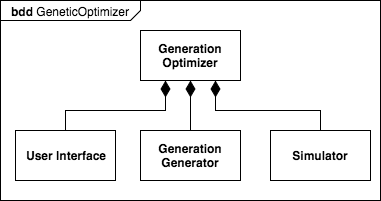
\includegraphics[width=0.7\linewidth]{../diagrams/bdd.png}
	\caption{BDD of the system.}
	\label{fig:bdd}
\end{figure}

The internal connections can be seen in the internal block diagram (IBD) in figure \ref{fig:ibd} and displays a greater level of information about which components are needed to run the algorithm. We see that \emph{GenerationGenerator} consists of two different parts, a generator and an interpreter of the random numbers. The point of the interpreter of the random numbers is, that it buffers the numbers such that there is always an amount of random numbers available.

\begin{figure}[h!]
	\centering
	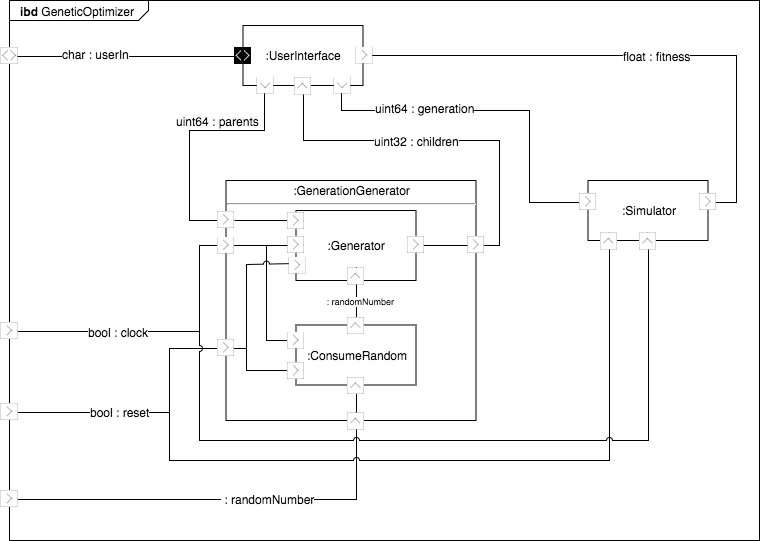
\includegraphics[width=\linewidth]{../diagrams/ibd.png}
	\caption{IBD of the system.}
	\label{fig:ibd}
\end{figure}

The functional behavior of the system can be described in a activity diagram, as seen in figure \ref{fig:activity}, where the different elements of the system are described. The user invokes the application by setting parameters $a$ and $b$ for the Rosenbrock function, after which we initialize the initial generation and evaluate it for $P(0)$. If the stopping criterion, which can be set by the user, is then met, this generation $P(0)$ is the final generation and thus saved before an application exit. If the stopping criterion is not met, GenerationGenerator will generate a generation $P(1)$ and mutates it following semantics previously described in section \ref{sec:theory}. For each generation, the fitness is display to the user. The algorithm continues iteratively.

\begin{figure}[h!]
	\centering
	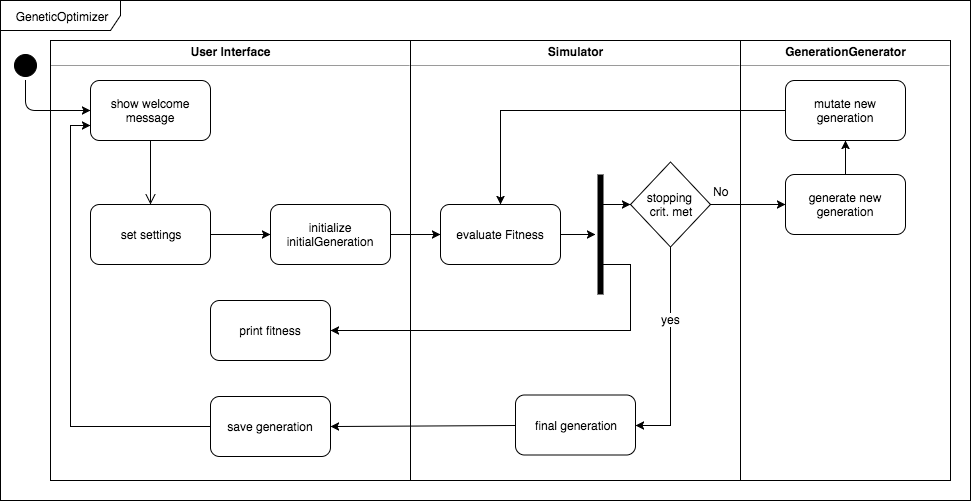
\includegraphics[width=0.9\linewidth]{../diagrams/overallActivity.png}
	\caption{Activity diagram for the system.}
	\label{fig:activity}
\end{figure}

The implementation has a number of potential allocations. Figure \ref{fig:allocation} shows one of them, as both the GenerationGenerator and Simulator are mapped to hardware. We decide not to allocate the user interface to hardware for simplicity purposes, however other possible allocations exist. We shall explore these options in the design phase using HLS and evaluate on their application in the results:

\begin{itemize} 
	\item Both the GenerationGenerator and Simulator are placed in software (a ARM Cortex-A9 processor).
	\item The GenerationGenerator is placed and accelerated in hardware (FPGA) and the Simulator is placed in software only (ARM Cortext-A9)
	\item The GenerationGenerator is put in software (ARM Cortext-A9) and the Simulator is put in hardware (FPGA).
\end{itemize}

Ideally, the computational generation of a new chromosome set (generation $P(k)$) and its simulation should run in real-rime. Therefore it is interesting to look at accelerating these parts using hardware and the FPGA, thus use the allocation shown in figure \ref{fig:allocation}.

\begin{figure}[h!]
	\centering
	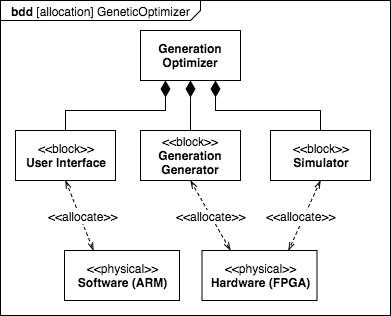
\includegraphics[width=0.9\linewidth]{../diagrams/allocation.png}
	\caption{Allocation diagram of a possible allocation of the system.}
	\label{fig:allocation}
\end{figure}

\subsection{Software design}
\begin{framed}
4. Design the software and apply design patterns that are suitable for your project, and motivate the choice of the used patterns. Use the Two-Part Architecture Model if relevant for the problem. Use the abstract OS package for the ZYBO board
\end{framed}

The user application software is built using the GoF State pattern in a concurrent construct with events invoked by the user and system components for changing states using the command pattern. We chose to encapsulate logic in states as they easily distinguish functionality and clearly represent transitions from one to another. Figure \ref{fig:statemachine} displays a finite state machine diagram implemented in C++ for the user application, where we use two concurrent states. One is for loading random numbers in a continuous flow and the other is the algorithm optimizer, as the generator uses the random numbers to create new chromosomes.

\begin{figure}[h!]
	\centering
	\includegraphics[width=0.9\linewidth]{../diagrams/statemachine.png}
	\caption{A state machine diagram of the user application.}
	\label{fig:statemachine}
\end{figure}

The optimizer state is quite bigger. It is made up of four different states where one is a nested state with two additional.
States transitions are triggered by commands specified as triggers trigger in the diagram and transitions handled by the states. State \textbf{Idle} is a waiting state where the user resides when they enter or when an optimization is done, aborted or when setup has concluded. The \textbf{Save} state is used to save the set generation of chromosomes which have been optimized. This is done using a simple print to the terminal. The \textbf{Setup} state allows the user to set parameters $a$ and $b$ for the Rosenbrock function, which stopping criterion and a initial generation. The \textbf{Optimize} state is a nested state machine where most of the algorithm is computed. It initiates in state \emph{Simulate}, where it calculates the fitness of a generation, then changes to either \textbf{Idle} or \textbf{GenerateGeneration} depending on the stopping criterion. It continues operations inside these until it has stopped or until aborted.

Figure \ref{fig:classdiagram} shows how we implemented the state design in C++ and on the Zybo board. Notice the \textbf{Context} holds the current state of the program, as well as best generation of chromosomes so far and the latest fitnesses. When the user invokes a command, we create actions of class \textbf{Action} of some specific task and call $HandleInput()$ on the context. It then delegates the concrete action to its current state, which calls $HandleAction()$ derived from the superclass \textbf{State}. Enter and exit methods are made when a state is entered or left.

\begin{figure}[h!]
	\centering
	\fbox{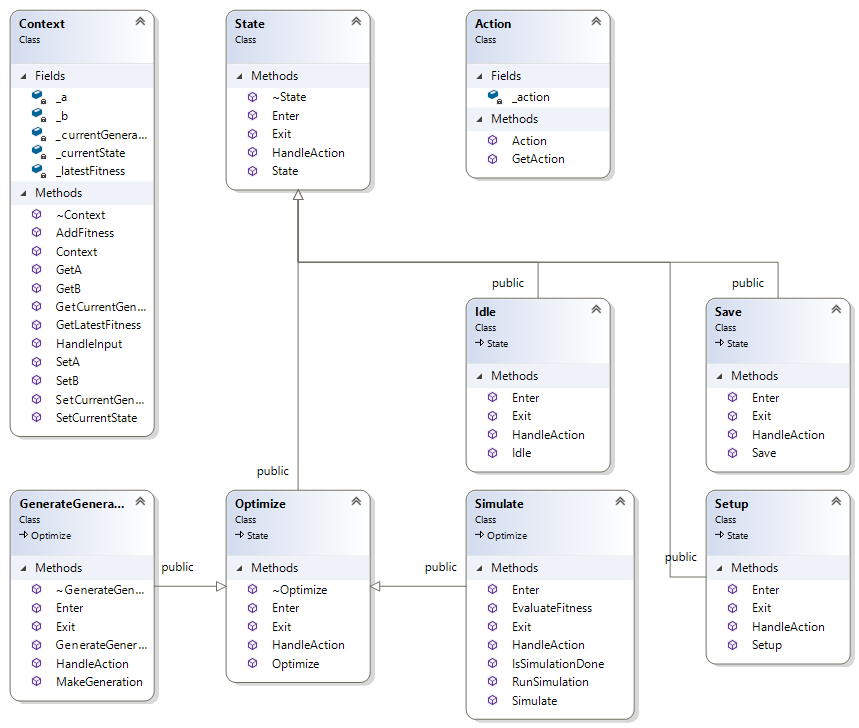
\includegraphics[width=0.9\linewidth]{../diagrams/ClassDiagram.png}}
	\caption{A class diagram of all the states in the user application, their inheritance and methods.}
	\label{fig:classdiagram}
\end{figure}

For implementing the concurrency control, a OS abstraction library is used. This is a wrapper for the functions defined in FreeRTOS, as we simply define two threads to control their respective part of the state diagram. See appendix A for more details.


